\chapter{Implementation of RoboMission}
\label{chap:implementation-of-robomission}

\itquote[0mm]{
A programmer is ideally an essayist who works with traditional aesthetic and literary forms as well as mathematical concepts, to communicate the way that an algorithm works and to convince a reader that the results will be correct.
}{D. E. Knuth}

% EXT:
%In the description of implementation, we focus on the aspects that are
%specific for system for learning programming, such as task representation,
%and transformation between programming blocks and code.

We present the overall architecture of RoboMission,
and describe aspects specific to the system for learning programming.
We intentionally avoid discussing details of used technologies,
which would make the text obsolete soon.
An overview of technologies used in the project is included as \cref{chap:technologies}.

\section{System Architecture}

RoboMission has a client-server architecture
with a fat frontend client communicating with the server via REST API
\cite{rest-api}.
In addition to the frontend app and backend services,
there are two other parts of the system:
scheduled jobs, which run periodically every week (e.g. metrics computation),
and tools for offline analysis of collected data
(e.g. Jupyter Notebooks). % templates).
% TODO: and "helper functions"
% TODO: ref/cite human-in-the-loop principle
% TODO: consider: list the parts in itemize
% TODO: other potential parts (future):
% - tasks/content management tools (CLI+browser)
% - simulations (CLI+browser)
% TODO: consider to include FE and BE sections below as subsections of this section
%TODO: diagram of overall architecture (client-server, communication, monitoring, scheduled jobs, offline analysis)

% \section{Frontend}
The frontend is a single page application with a \emph{redux architecture}
\cite[ch.\,12]{flux},
which means that a single immutable state stores all application data.
% The state cannot be mutated directly;
A new state can be created only by dispatching an action.
Each part of the state then defines its \emph{reducer},
a pure function that takes a state and an action, and returns a new state.
% ... and the only way the state can be changed is by dispatching actions.
% ... dispatcher then takes dispatched actions one by one and reduce them (notifying
%     connected containers about the new state)
% ... reducers: state, action -> new state (pure functions)
% "unidirectional UI" (as opposed to MVC and similar architectures)
The view is then assembled using declarative reusable
components, that are
either \emph{presentational} (e.g. describing how the game world is
rendered), or \emph{behavioral} (selecting data from the state, % to use for the rendering,
and dispatching actions) \cite{react}. %  and their triggers.
The application also defines a few asynchronous workflows (\emph{sagas}),
e.g. for program interpretation, and task solving process. %, or sending events to Google Analytics.  % better examples?
%% TODO: at least one sentence about React components?
%\subsection{React Components}
%
%\begin{itemize}
%\item mostly declarative - simple mental model: rebuilding from scratch every time anything change -> less error prone
%\item reusability -> use of single component on many places in different contexts,

%% TODO: Improve the diagram to make a point; otherwise remove.
%\imgW{frontend-dependencies}{%
%  Frontend modules/packages and dependencies between them.}
% TODO: Give examples of (in description) of what are submodules inside core, utils, reducers, sagas, containers, components.
% TODO: Note that some dependencies are eliminated via dependency injection in
  % redux-architecture (+ example!)
% TODO: Improve diagram, use a standard notation (see slides from Software Engineering)
% TODO: Explain the difference between component and containers.

%TODO: redux-architecture (data+events flow) diagram (specifically for our app) (and show how the flow of events is easier to reason about in React+Redux (than in Angular)).

%% TODO: at least one sentence about React components?
%\subsection{React Components}
%
%\begin{itemize}
%\item mostly declarative - simple mental model: rebuilding from scratch every time anything change -> less error prone
%\item reusability -> use of single component on many places in different contexts,
%  or even outside the app (use space-world for ai-search-workshop)
%\item example from our codebase (code, image)
%\end{itemize}

% TODO: This might be relevant if shown for code interpretation instead of
% sending feedback.
%\subsection{Asynchronous Side Effects}
%\label{sec:robomission-asynchronous-side-effects}
%
%Frontend applications are usually full of asynchronous side effects
%(e.g. fetching data from server, wating for user actions).
%Many ways to handle them were proposed,
%such as callbacks (REF) or promises (REF).
%%The most basic one are callbacks --
%%asychronous function takes a function (``callback'') as a parameter
%%and calls it once the asynchronous action is resolved.
%%(TODO: mention/explain promises -- advantage: very explicit; clean error
%%handling; show example for data fetching)
%
%However, both callbacks and promises become awkward for expressing complex
%asynchronous flows, such as visualizing code execution,
%leading to unreadable ``callback hell''. % TODO: ref for callback hell
%Sagas provide an alternative way of handling asynchronous effects using generators.
%Instead of performing asynchronous effects directly, sagas yield
%descriptions of such effects.
%As an example, there is a saga responsible for processing
%submitted feedback.
%Note that while the code contains many asynchronous effects,
%it can be read nearly as easy as standard linear synchronous code.
%
%% TODO: insert comments in the code
%% TODO: mention other advantage of sagas - great testability
%% TODO: also mention new async-await concept
%
%\begin{lstlisting}[language=ES6]
%// Generator for a single submit-feedback request
%function* submitFeedback(action) {
%  const { text, email } = action.payload;
%  // Asynchronous request to get a value from state
%  const url = yield select(getFeedbackUrl);
%  try {
%    // Asynchronous request to post data to server
%    yield call(api.sendFeedback, url, text, email);
%    // Asynchronous request to dispatch a new action
%    yield put(actions.submitFeedback.success());
%  }
%  catch (error) {
%    const { fieldErrors } = error;
%    yield put(
%      actions.submitFeedback.failure(fieldErrors));
%  }
%}
%\end{lstlisting}

% TODO: add code samples for each concept (react component + image, reducer, saga)
% TODO(optional): awesome ES6 (example from our code)
% TODO(Material Design): example of our component + code

% \section{Backend}

%\begin{itemize}
%\item Django, Django Rest Framework
%\item django apps (python packages): learn, monitoring (potential diagram for planned architecture: users, tasks, learn, adaptability, monitoring, simulations, analysis)
%\item models (...), serializers, views, services/use cases/core
%\item data export
%\item monitoring app, metrics computation
%\item generators (e.g. metric computation)
%\item architecture (of individual apps): viewsets/management, services,
%serializers, models, core (actions, credits, recommendation)
%\end{itemize}

% TODO?: more about the relationship between the backend and ALS components
% (domain, student, tutor, UI, analysis layer)
The backend is decomposed into modules defining database entities,
their serializers (JSON for sending data to the frontend, CSV for exports),
\emph{view sets} describing REST API, % TODO: cite view-sets
and core modules with mostly pure functions
for computing performance, skills, and recommendations.
% NOTE: It would make sense to decompose to packages corresponding to
% the ALS components: domain, student, tutor, ui, monitoring, analysis.
% TODO: + domain parsing, monitoring.
%Technologies are becoming obsolete soon,
%so will not discuss them in the text.
% Source code of the project attached ... \cref{sec:attachment.source-code}

\section{Domain Representation}

The domain is represented by a JSON file containing all problem sets %missions, phases, and
and relationships between them, as well as their setting (e.g. which toolbox to use)
and names of their tasks.
Each task is then described in a separate file (\cref{sec:impl.task-sources}).
Furthermore, there is a separate JSON file containing values for parameters
of domain entities (e.g. a time threshold for good performance for each task).
%EXT:
%It is convenient to have the relationships and the parameters in different files,
%because the former is currently edited by people, while the latter is
%a result of a computation.

\subsection{Task Sources}
\label{sec:impl.task-sources}

Each task is described by a single file in a markdown-based format \cite{markdown},
containing its name, setting, and solution.
Task sources in markdown files have several advantages: % as opposed to have them in DB
they are human readable,  % + rendered by GH to a nicer presentation
each change is version-controlled,
and the task can be edited easily in any text editor.
\Cref{fig:task-source} shows a high-level grammar for task description,
together with an example.

% There is also top-level [- option: value]*, currently not used
\begin{figure}[htb]
\centering
\begin{subfigure}{.49\textwidth}
{\lstset{numbers=none, showlines=true}
\begin{lstlisting}[basicstyle=\small\ttfamily]
# <name>

## Setting
```
<SpaceWorld>
```

[- option: value]*


## Solution
```
<RoboCode>
```


\end{lstlisting}}
\caption{High-level grammar}
\end{subfigure}
\begin{subfigure}{.49\textwidth}
{\lstset{numbers=none}
\begin{lstlisting}[basicstyle=\small\ttfamily]
# turning-left

## Setting
```
|bM|b |b |bM|b |
|kA|k |kM|k |kA|
|k |k |kA|kM|k |
|kM|k |kS|k |kA|
```

## Solution
```
left()
fly()
fly()
```
\end{lstlisting}}
\caption{Turning Left (rendered in \cref{fig:robomission-task1})}
\end{subfigure}
\caption{Task source grammar and an example.}
\label{fig:task-source}
\end{figure}

Currently, there are only two setting options: length and energy limits.
\texttt{SpaceWorld} and \texttt{RoboCode} fragments follow their own grammars, which
are described in \cref{sec:impl.spaceworld,sec:robocode}.
% [consider] Markdown files are then parsed and loaded into DB by a single command.
% [consider]
% - Localized task names are not part of the task source,
% because all localized messages live on the same place in a single file on FE.
% - PEG grammar for parsing
% - internal represenation (DB model and its serializers for FE and for CSV exports)

\subsection{Space World Description}
\label{sec:impl.spaceworld}

% TODO: Unify "game world" -- "space world
Each Space World (\cref{sec:robomission.game-world}) is described by a simple
human-readable string.
See \cref{fig:spaceworld-in-editor} for an example and description.
Set of valid Space World descriptions is given by the
following context-free grammar:

\begin{lstlisting}
SpaceWorld -> Row+
Row -> '|'(Field'|')+ EOL  // EOL = End Of Line
Field -> Background Object*
Background -> 'r' | 'g' | 'b' | 'y' | 'k'
Object -> 'S' | 'A' | 'M' | 'D' | 'W'
\end{lstlisting}


%\begin{figure}[h]
%\begin{center}
%\begin{subfigure}{.4\textwidth}
%\centering
%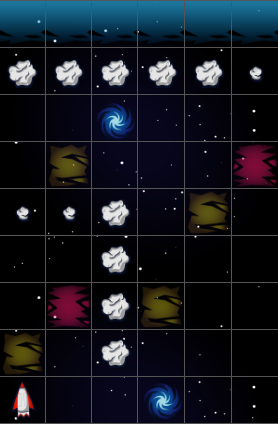
\includegraphics[width=.9\textwidth]{img/spaceworld}
%\end{subfigure}
%\begin{subfigure}{.36\textwidth}
%\centering
%{\lstset{numbers=none}
%\begin{lstlisting}
%|b |b |b |b |b |b |
%|kA|kA|kA|kA|kA|kM|
%|k |k |kW|k |k |k |
%|k |y |k |k |k |r |
%|kM|kM|kA|k |y |k |
%|k |k |kA|k |k |k |
%|k |r |kA|y |k |k |
%|y |k |kA|k |k |k |
%|kS|k |k |kW|k |k |
%\end{lstlisting}}
%\end{subfigure}
%\end{center}
%\caption{Example of Space World with its source code. TODO: Describe letters; consider replacing code listing with a screenshot from task editor with code highlighting}
%\label{fig:spaceworld-source}
%\end{figure}


\imgW[0.7]{spaceworld-in-editor}%
{Example Space World with its description. % source code.
Each line represents one row of the grid
and is split by pipes (``|'') into fields.
Each field starts with a lower-case letter denoting color of the field
(e.g. b = blue, k = black),
followed by an optional upper-case letter denoting an object
(A = asteroid, S = spaceship, etc.).
For example, ``rD'' is a red field with a diamond.}



\section{RoboCode}
\label{sec:robocode}

\emph{RoboCode} is a Python-like programming language
for representing solutions in task sources.
It closely corresponds to the text written on Blockly blocks
with a few exceptions, such as %added parentheses
shorter function names and added parentheses
(e.g. \texttt{left()} instead of \texttt{fly left}).
% also: fly right -vs- fly()
% and abbreviated literals (e.g. ``b'' instead of ``blue'').
% difference: parenthesis (color() vs. color) and literals ('b' vs. blue)
% TODO: check the statement above
It is also intended to be used in more advanced problem sets as the
transitional phase from block-based to text-based programming.
The language was designed % with the following requirements in mind:
to be simple for beginners, understandable without its previous knowledge,
concise (short, but readable programs),
and matching Python closely (for an easy transition to Python).

%\subsection{Syntax and Semantic}
%\label{sec:syntax-semantic}

% TODO[consider] note on mixing lexer+parser+some semantic analysis
% (which is partially convenient, partially confusing)

There are four basic commands: % for performing actions:
\texttt{fly()},
\texttt{left()},
\texttt{right()}, and
\texttt{shoot()}.
%\begin{lstlisting}
%fly()
%left()
%right()
%shoot()
%\end{lstlisting}
Each action is combined with moving one row forward.
The movement takes place after the action, with the exception of left and right turning actions, where the movement and the action happen simultaneously,
i.e. the spaceship flies diagonally to the left or to the right.
% TODO: Rephrase. Is confusing, because the general statement ("movement takes
% place after the action") is only relevant for shoot(), and all the other
% commands are special cases.

Loops and conditional statements are same as in Python,
with an exception of the repeat loop,
which was simplified % to a form
% matching a corresponding Blockly block, which is
to be easier to understand: % by beginners:
% TODO: ass robocode highlighting
\begin{lstlisting}
repeat 4:
    fly()
\end{lstlisting}

Conditions %inside while-loops and if-statements
are restricted to the following forms.
% (again in order to match the respective Blockly blocks):
(Color codes are same as in the Space World description,
i.e. 'r' is red, 'g' is green' etc.)
% (again in order to match the respective Blockly blocks):
\begin{lstlisting}
position() [==|!=|>|<|>=|<=] [1..6]
color() [==|!=] ['r'|'g'|'b'|'y'|'k']
<test> [and|or] <test>
\end{lstlisting}
Control structures can nest arbitrarily:
% TODO: Program for solvint the task from the previous section
%       (change either the program, the task, or both).
%\begin{figure}[h]
\begin{lstlisting}
while color() != 'b':
    if position() == 1:
        right()
    if position() >= 4:
        shoot()
    fly()
\end{lstlisting}
%\caption{Example of a complete RoboCode program}
%\label{fig:robocode-example}
%\end{figure}


\subsection{RoboAST}

While Python-like RoboCode is convenient for writing sample solutions,
a more compact form would be better for logging, storing in DB and analysis.
Secondly, a block-based presentation of the code is needed for students.
Last but not least, a JavaScript equivalent of the code is useful for
interpreting the code in the browser.
\Cref{tbl:code-representation} shows an overview of all representations.


\begin{table}[htb]
\centering
\caption{Different code representations used within the system.}
\begin{tabular}{l l l}
\toprule
Name & Form & Usage  \\
\midrule
RoboCode     & text (Python-like) & sample solutions in task sources  \\
MiniRoboCode & text (compact) & logging, storing in DB, analysis  \\
RoboBlocks   & blocks (Blockly) & code editor for students  \\
RoboJS       & text (JavaScript) & interpretation in browser  \\
RoboAST      & JSON (AST) & intermediate representation \\
\bottomrule
\end{tabular}
\label{tbl:code-representation}
\end{table}

% TODO: [consider] Use "presentation" for the "fringe" representations.
% (Because it is confusing to talk about common representation of representations.)
To avoid implementing separate transformations between each pair of these
representations, we introduced a common intermediate representation,
\emph{RoboAST}, which is an %simple
\emph{Abstract Syntax Tree} \cite{ast} in JSON
(\cref{fig:robocode-transformations-example}).
For each of the four other representations, it is enough to implement
its parser returning RoboAST object, and
its generator from RoboAST (\cref{fig:robocode-transformations}).
With a parser and a generator for each representation,
%it is possible to transform representation A
%into representation B by parsing A into RoboAST and
%then generating B from this RoboAST.
any representation A can be transformed into any representation B
by first parsing A into RoboAST and then generating B from this RoboAST.
% "This mechanism ..."
% TODO: mention the disadvantage - not able to use functionality provided by Blockly (code generators)

% TODO: fix the image (missing black line on right) (+ make it lower: tree-like
% structure, with RoboAST as a root at the top.)
\imgW[0.6]{robocode-transformations}{Transformations between RoboAST and other representations.}

\imgW{robocode-transformations-example}{Example of a RoboAST (in the middle),
  and corresponding RoboBlocks, RoboCode, MiniRoboCode, and RoboJS.}


\subsection{Parsing Expression Grammar}

For parsing RoboCode into RoboAST, we use a \emph{parsing expression grammar}
(PEG) \cite{peg}.
% TODO: verify the following statement
PEGs are essentially unambiguous context-free grammars with prioritized rules
and more compact syntax.
% and lookahead expressions (TODO: example).  % using our grammar - if we don't
% use it, then don't mention it.
% TODO: check grammar (should ... be transformed)
The PEG implementation we use%
\footnote{PEG.js, available at \url{https://pegjs.org}.}
allows to define a \emph{match result} for each parsed subexpression,
using an arbitrary JavaScript code returning a subtree of the final AST.
For illustration, there are
two % a few
examples of RoboCode parsing rules:

\begin{lstlisting}
CompoundStatement = IfStmt / WhileStmt / RepeatStmt
WhileStmt = "while" __ t:Test ":" b:Body
  { return { head: "while", test: t, body: b } }
\end{lstlisting}
%Test
%  = CompoundTest
%  / SimpleTest

PEGs can be parsed in linear time, they do not require a separate lexer,
and the resulting grammar is readable and concise;
the PEG for RoboCode % (as described in \cref{sec:syntax-semantic})
has only about 100 lines. % of code.
However, a preprocessing of the RoboCode is necessary, because
PEGs are context-free,
while RoboCode is a context-sensitive language
-- the context is created by indentation.
In addition, it is also useful to store line numbers alongside the statements
to enable \emph{meta-interpreting},
such as showing executed line, or linking errors to the point in the source code.
Therefore, the preprocessing step transforms the code in a context-free form,
in which each line of the code is prepended corresponding line number,
and adding and removing indentation levels is denoted by \texttt{\{}
and \texttt{\}} characters respectively.
For example, the preprocessed code for the program shown in
\cref{fig:robocode-transformations-example} would be:
\begin{lstlisting}
1| shoot()
2| repeat 4:
{
3| right()
4| left()
}
\end{lstlisting}
% The \cref{fig:robocode-transformations-example} also shows the final RoboAST object.

\subsection{MiniRoboCode}
\label{sec:minirobocode}

MiniRoboCode is a condensed form of the RoboCode.
It replaces indentation by curly brackets,
keywords and functions by their first letters,
and removes whitespace characters
in order to fit programs into a single short line.
The mapping from the RoboCode is described by the following rules:
% shown in \cref{fig:minirobocode-transformation-rules}.
\smallskip

\noindent\begin{minipage}{.49\textwidth}
\begin{lstlisting}[numbers=none]
repeat --> R
while --> W
if --> I
else --> /
position() --> x
== --> =
\end{lstlisting}
\end{minipage}\hfill
\begin{minipage}{.49\textwidth}
\begin{lstlisting}[numbers=none]
fly() --> f
left() --> l
right() --> r
shoot() --> s
color == 'y' --> y
color != 'y' --> !y
\end{lstlisting}
\end{minipage}

%\begin{figure}[h]
%\begin{subfigure}{.49\textwidth}
%{\lstset{numbers=none}
%\begin{lstlisting}
%repeat --> R
%while --> W
%if --> I
%else --> /
%position() --> x
%== --> =
%\end{lstlisting}}
%\end{subfigure}
%\begin{subfigure}{.49\textwidth}
%{\lstset{numbers=none}
%\begin{lstlisting}
%fly() --> f
%left() --> l
%right() --> r
%shoot() --> s
%color == 'y' --> y
%color != 'y' --> !y
%\end{lstlisting}}
%\end{subfigure}
%%\caption{Transformation rules from RoboCode to MiniRoboCode. (In reality, the transformations goes through RoboAST.)}
%%\label{fig:minirobocode-transformation-rules}
%\end{figure}
% \Cref{fig:minirobocode-transformations} shows
\smallskip

\noindent
Two examples of complete transformations into MiniRoboCode:
\smallskip

\noindent\begin{minipage}{.49\textwidth}
\begin{lstlisting}[numbers=none]
fly()
while color() == 'b':
    left()
    right()
fly()
<*\arrowlinesplit*>
fWb{lr}f
\end{lstlisting}
\end{minipage}\hfill
\begin{minipage}{.49\textwidth}
\begin{lstlisting}[numbers=none]
repeat 6:
    if position() > 1:
        shoot()
    else:
        right()
<*\arrowlinesplit*>
R6{Ix>1{s}/{r}}
\end{lstlisting}
\end{minipage}
\smallskip

%\begin{figure}[h]
%\begin{subfigure}{.49\textwidth}
%{\lstset{numbers=none}
%\begin{lstlisting}
%fly()
%while color() == 'b':
%    left()
%    right()
%fly()
%-------------------
%fWb{lr}f
%\end{lstlisting}}
%\end{subfigure}
%\begin{subfigure}{.49\textwidth}
%{\lstset{numbers=none}
%\begin{lstlisting}
%repeat 6:
%    if position() > 1:
%        shoot()
%    else:
%        right()
%-------------------
%R6{Ix>1{s}/{r}}
%\end{lstlisting}}
%\end{subfigure}
%%\caption{Examples of transformations of RoboCode to MiniRoboCode.}
%%\label{fig:minirobocode-transformations}
%\end{figure}

MiniRoboCode is useful not only for logging and storing programs in the database,
but also for many analyses, because it is easy to process by counting
letters or matching simple regular expressions, and because they are short
enough to be used as labels in plots.


\subsection{RoboBlocks}

Blockly%
\footnote{Available at \url{https://developers.google.com/blockly/}.}
is an implementation of block-based programming
environment from Google,
which we use in the code editor for students
(shown e.g. in \cref{fig:robomission-task1}).
% TODO: ref to section about block-base programming envs and their pros/cons
% TODO: mention advnatages of using Blockly from Google: well-tested, widely-used
% (and disadvantage: don't play nicely with modern JS workflow; sometimes needs
% awful hacks to digging in the source code to achieve a desiered behavior
Blockly allows to import and export the currently assembled program in
an XML format, that we call \emph{RoboBlocksXML}
%(See \cref{fig:roboblocks-xml} for an example of the XML.)
(\cref{fig:roboblocks-xml}).
Both transformations between RoboBlocksXML and RoboAST are straightforward.

% TODO(opt): some details about Blocly? (definition of blocks)
%  (or just overview of currently used blocks (in a row "toolbox" to save space)

% TODO: make it just refferable listing, instead of figure
\begin{figure}[h]
\begin{lstlisting}[basicstyle=\small\ttfamily]
<xml xmlns="http://www.w3.org/1999/xhtml">
 <block type="start">
  <next><block type="shoot">
   <next><block type="repeat">
    <field name="count">4</field>
    <statement name="body">
     <block type="fly">
      <field name="direction">right</field>
      <next><block type="fly">
       <field name="direction">left</field>
      </block></next>
     </block>
    </statement>
   </block></next>
  </block></next>
 </block>
</xml>
\end{lstlisting}
  \caption{%
    RoboBlocksXML for the program shown in %
    \cref{fig:robocode-transformations-example}.}
\label{fig:roboblocks-xml}
\end{figure}

As the RoboBlocks are used by children, it is important to use localized labels
on the blocks.
Depending on the language domain, we initialize Blockly blocks with the corresponding
version of localized block labels
(\cref{fig:roboblocks-english-czech}).
%(See \cref{fig:roboblocks-english-czech} for an example of the same program in two languages.)
%Blockly supports its own localization mechanism that fits well
%within the localization framework used in our project.

\imgW[0.5]{roboblocks-english-czech}{Same program in English and Czech localizations of RoboBlocks.}
% TODO: Fix the image so that both images are of the exactly same size and sharpness.

\subsection{RoboJS and Interpretation}
\label{sec:robomission-robojs}

Instead of implementing our own interpreter of RoboCode,
we transform the code through RoboAST into JavaScript,
%(described in \cref{sec:robomission-robojs})
and then use a JavaScript interpreter to run the code.
The generated \emph{RoboJS} % is just a JavaScript that
assumes to be executed within a
context providing hooks for functions corresponding to actions (\texttt{fly}, \texttt{left}, \texttt{right}, \texttt{shoot}),
sensors (\texttt{color}, \texttt{position}),
and meta-interpreting (\texttt{isStopped}, \texttt{highlightBlock})
(\cref{fig:robojs-example}).

The interpreter does not have to be necessary a \emph{JavaScript} interpreter,
since it is easy to transform RoboAST to any other common imperative language.
% (at least to the common imperative languages).
However, the interpreter must satisfy the following requirements:
% TODO: check grammar: "to be implemented ... to allow ..."?
be implemented in JavaScript (to run in the browser),
allow to define custom asynchronous hooks
(to perform actions),
%(in order to perform actions, sensor measurements, and block highligting),
and allow to step the code, or at least to impose a limit on
the number of steps % or time
(to break infinite loops).
%(in order to break infinite loops).
% interprets a language that can be generated easily from the RoboAST (which includes most languages),
%There is nothing special about using JavaScript as the language being interpreted,
%other that the JS-interpreter satisfies all our requirements
%and is relatively simple to use.

% We could use any interpreter that would satisfy the following conditions:
%\begin{enumerate}
%\item is implemented in JavaScript (in order to run in the browser),
%\item interprets a language that can be generated easily from the RoboAST
%  (which includes most languages),
%\item allows to define custom asynchronous hooks
%  (needed for actions, sensors, and block highligting),
%\item allows to step the code, or at least to impose a step or time limit
%  (in order to break infinite loops).
%\end{enumerate}
% TODO(opt): why not to use JS interpreter in browser: safety (sandbox requirement)
% + probably also not able to step the code or set the time limit, but I haven't verified this


%For the interpretation of the student code yet another representation is needed,
%a JavaScipt code that can be fed into a JS interpreter.
%(See \cref{sec:robomission-interpretation} for the details of the interpretation).


\begin{figure}[h]
\begin{subfigure}{.28\textwidth}
\centering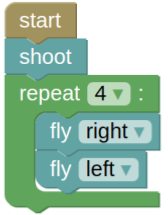
\includegraphics[width=.8\textwidth]{img/roboblocks-english}
\end{subfigure}
\begin{subfigure}{.7\textwidth}
{\lstset{numbers=none}
\begin{lstlisting}
highlightBlock(1);
shoot();
highlightBlock(2);
for (var i1_ = 0; i1_ < 4; i1_++) {
  highlightBlock(3);
  right();
  highlightBlock(4);
  left();
}
\end{lstlisting}}
\end{subfigure}
\caption{%
  Example of a RoboJS (right) for given RoboBlocks program (left). %
  % Repeat loops require to generate unique names for iteration variables.
  Each original command is accompanied by \texttt{highlightBlock(blockId)},
  so that the meta-interpreter knows which block to highlight.}
\label{fig:robojs-example}
\end{figure}

%We have not implemented a parser from RoboJS to RoboAST,
%simply because we do not need this tranformation;
%otherwise, there is no technical obstacle and the parser would be based on a similar PEG gramamar as for the RoboCode.

We use an existing JavaScript interpreter%
\footnote{JS-interpreter, available at \url{https://github.com/NeilFraser/JS-Interpreter}.}
and wrap it into two
additional layers: the first layer is a generator
that yields actions, sensor requests and
meta-interpreting effects (e.g. block highlighting), % checking for interruption).
and the second layer is a saga
%(see \cref{sec:robomission-asynchronous-side-effects})
that handles all these asynchronous effects.
The separation into these two layers allows to test the interpreter logic
easily without dealing with asynchronous effects.
